%==============================================================================
% Sjabloon onderzoeksvoorstel bachproef
%==============================================================================
% Gebaseerd op document class `hogent-article'
% zie <https://github.com/HoGentTIN/latex-hogent-article>

% Voor een voorstel in het Engels: voeg de documentclass-optie [english] toe.
% Let op: kan enkel na toestemming van de bachelorproefcoördinator!
\documentclass{hogent-article}

% Invoegen bibliografiebestand
\addbibresource{voorstel.bib}

% Informatie over de opleiding, het vak en soort opdracht
\studyprogramme{Professionele bachelor toegepaste informatica}
\course{Bachelorproef}
\assignmenttype{Onderzoeksvoorstel}
% Voor een voorstel in het Engels, haal de volgende 3 regels uit commentaar
% \studyprogramme{Bachelor of applied information technology}
% \course{Bachelor thesis}
% \assignmenttype{Research proposal}

\academicyear{2024-2025} % TODO: pas het academiejaar aan

% TODO: Werktitel
\title{Het implementeren van Internet of Things (IoT) om de wachttijden voor patiënten in de afdeling Accident and Emergency (A\&E) van de National Health Service (NHS) te verkorten.}


% TODO: Studentnaam en emailadres invullen
\author{Brahim Mahfoudhi}
\email{Brahim.Mahfoudhi@student.hogent.be}

% TODO: Medestudent
% Gaat het om een bachelorproef in samenwerking met een student in een andere
% opleiding? Geef dan de naam en emailadres hier
% \author{Yasmine Alaoui (naam opleiding)}
% \email{yasmine.alaoui@student.hogent.be}

% TODO: Geef de co-promotor op
\supervisor[Co-promotor]{S. Beekman (Synalco, \href{mailto:sigrid.beekman@synalco.be}{sigrid.beekman@synalco.be})}

% Binnen welke specialisatierichting uit 3TI situeert dit onderzoek zich?
% Kies uit deze lijst:
%
% - Mobile \& Enterprise development
% - AI \& Data Engineering
% - Functional \& Business Analysis
% - System \& Network Administrator
% - Mainframe Expert
% - Als het onderzoek niet past binnen een van deze domeinen specifieer je deze
%   zelf
%
\specialisation{Mobile \& Enterprise development}
\keywords{Scheme, World Wide Web, $\lambda$-calculus}
\begin{document}

\begin{abstract}
%  Hier schrijf je de samenvatting van je voorstel, als een doorlopende tekst van één paragraaf. Let op: dit is geen inleiding, maar een samenvattende tekst van heel je voorstel met inleiding (voorstelling, kaderen thema), probleemstelling en centrale onderzoeksvraag, onderzoeksdoelstelling (wat zie je als het concrete resultaat van je bachelorproef?), voorgestelde methodologie, verwachte resultaten en meerwaarde van dit onderzoek (wat heeft de doelgroep aan het resultaat?).
De wachttijden voor Accident and Emergency (A\&E) behandelingen binnen de National Health Service (NHS) in Engeland hebben over de vele jaren een continu opwaartse trend vertoond. Ondanks de systematische steun van de Britse overheid heeft de National Health Service (NHS) nog geen oplossing kunnen vinden voor dit probleem. Patiënten maken zich ernstige zorgen over de triagewachttijden, worden onopzettelijk genegeerd en verergeren bestaande medische aandoeningen tijdens het wachten, wat kan leiden tot ernstige complicaties. Om die reden richt dit onderzoek zich op het beantwoorden van de volgende vraag: Kan Internet of Things (IoT) geïmplementeerd worden om de wachttijden verminderen en de efficiëntie van de zorgverlening te verbeteren? Om deze vraag te beantwoorden, is het essentieel om een antwoord te geven op een aantal deelvragen. Ten eerste is het belangrijk om te achterhalen wat de onderliggende oorzaak is van de lange wachttijden, dit is een belangrijke vraag om te bepalen of IoT een geschikte oplossing kan zijn bij het verkorten van de wachttijden. Daarnaast is het van belang om te identificeren welke IoT-devices er nodig zijn om de onderliggende oorzaak te verhelpen. Tot slot is het noodzakelijk om de volgende vraag te beantwoorden: hoe kan er bewezen worden dat het IoT de wachttijd kan verkorten? Het onderzoek begint met het uitvoeren van een oorzaakanalyse, om een beter inzicht te krijgen in de oorzaak van de lange wachttijden binnen de A\&E-afdelingen van de National Health Service (NHS). Vervolgens zal er een gegevensverzameling van meerdere National Health Service (NHS) ziekenhuizen uitgevoerd worden, waarbij één ziekenhuis geselecteerd wordt volgens verschillende criteria. Na de selectieprocedure volgt er een casestudie, uitgevoerd over verschillende Internet of Things (IoT)-tech-no-lo-gieën die aanzienlijke voordelen bieden tegen langdradige wachttijden binnen de gezondheidszorg. Verder zal er een set van IoT-devices geïdentificeerd en geselecteerd worden door middel van de casestudie. Vervolgens volgt het genereren van synthetische data, deze data representeert een imitatie van de gegevens die verzameld zijn door de geselecteerde IoT-devices. De verworven gegevens, kennis en synthetische data voor het trainen van een Machine Learning- en Predictive analytics model, het Machine Learning model zal gebruikt worden voor het voorspellen of IoT een gunstige invloed heeft op de lange wachttijden, Het Predictive analytics model in daarentegen zal voorspellen of IoT een voordelig effect heeft op de langdurige wachttijden voor diverse scenario’s zoals een verschil in aantal patiënten en personeel. De bevindingen met betrekking tot de voorspellingen worden vervolgens vergeleken met de historische data, de waarnemingen die daaruit volgen worden vervolgens geanalyseerd in de context van potentiële voordelen van Internet of Things (IoT) met betrekking tot de uitgebreide Accident and Emergency (A\&E) wachttijden. De resultaten van het onderzoek lichten verder toe of Internet of Things (IoT) kan bijdragen bij het verminderen van wachttijden voor de Accident and Emergency (A\&E) afdeling door gebruik te maken van technologieën uit verschillende IoT categorieën. Als er voldoende aanwijzingen zijn dat Internet of Things (IoT)-tech\-no\-lo\-gieën een gunstige invloed hebben op de wachttijden binnen de Accident and Emergency (A\&E) afdeling, dan zijn de resultaten als succesvol gewaardeerd. Tot slot is het van belang om nadruk te leggen op het feit dat dit onderzoek zich enkel richt op het toepassen van Internet of Things (IoT) als benadering voor uitgebreide wachttijden, zonder consideratie te houden van de beveiliging en privacy risico's hiervan.
\end{abstract}

\tableofcontents

% De hoofdtekst van het voorstel zit in een apart bestand, zodat het makkelijk
% kan opgenomen worden in de bijlagen van de bachelorproef zelf.
%---------- Inleiding ---------------------------------------------------------

% TODO: Is dit voorstel gebaseerd op een paper van Research Methods die je
% vorig jaar hebt ingediend? Heb je daarbij eventueel samengewerkt met een
% andere student?
% Zo ja, haal dan de tekst hieronder uit commentaar en pas aan.

\paragraph{Opmerking}
Dit voorstel is gebaseerd op het onderzoeksvoorstel dat werd geschreven in het
kader van het vak Research Methods dat ik (vorig/dit) academiejaar heb
uitgewerkt (met medestudent Mohammed-Ali Kasraoui als mede-auteur).
 

\section{Inleiding}%
\label{sec:inleiding}

% Waarover zal je bachelorproef gaan? Introduceer het thema en zorg dat volgende zaken zeker duidelijk aanwezig zijn:

%\begin{itemize}
%  \item kaderen thema
%  \item de doelgroep
%  \item de probleemstelling en (centrale) onderzoeksvraag
%  \item de onderzoeksdoelstelling
% \end{itemize}
%
%Denk er aan: een typische bachelorproef is \textit{toegepast onderzoek}, wat betekent dat je start vanuit een concrete probleemsituatie in bedrijfscontext, een \textbf{casus}. Het is belangrijk om je onderwerp goed af te bakenen: je gaat voor die \textit{ene specifieke probleemsituatie} op zoek naar een goede oplossing, op basis van de huidige kennis in het vakgebied.

%De doelgroep moet ook concreet en duidelijk zijn, dus geen algemene of vaag gedefinieerde groepen zoals \emph{bedrijven}, \emph{developers}, \emph{Vlamingen}, enz. Je richt je in elk geval op it-professionals, een bachelorproef is geen populariserende tekst. Eén specifiek bedrijf (die te maken hebben met een concrete probleemsituatie) is dus beter dan \emph{bedrijven} in het algemeen.

%Formuleer duidelijk de onderzoeksvraag! De begeleiders lezen nog steeds te veel voorstellen waarin we geen onderzoeksvraag terugvinden.

%Schrijf ook iets over de doelstelling. Wat zie je als het concrete eindresultaat van je onderzoek, naast de uitgeschreven scriptie? Is het een proof-of-concept, een rapport met aanbevelingen, \ldots Met welk eindresultaat kan je je bachelorproef als een succes beschouwen?

%----------------------------------------------------------Inleiding-------------------------------------------------


De toenemende wachttijden voor behandelingen op de Accident and Emergency (A\&E) afdelingen binnen de National Health Service (NHS) \ref{fig:Figuur0} vormen een groeiend probleem in het Verenigd Koninkrijk en zijn daarom de oorzaak van veel discussie in de Britse media. Dit werd verder versterkt dankzij een recent onderzoek uitgevoerd door The Rt Hon. Professor the Lord Darzi of Denham, een lid van de House of Lords van het Verenigd Koninkrijk.

\subsubsection*{Probleemstelling}
Volgens de bevindingen uit het onderzoek zitten de A\&E afdelingen van de NHS in een “vreselijke staat”. De studie toont namelijk aan dat meer dan 100.000 kinderen vorig jaar meer dan 6 uur moesten wachten en dat bijna 10 procent van alle patiënten nu 12 uur of langer moet wachten om behandeld te worden \autocite{LordDarzi2024}. Deze langdurige wachttijden hebben serieuze consequenties voor patiënten. Volgens een toespraak over het onderzoek door de Britse Premier, Sir Keir Starmer, zijn de lange A\&E wachttijden niet alleen een bron van angst en bezorgdheid, maar leiden ook tot duizenden vermijdbare sterfgevallen. Volgens de Royal College of Emergency Medicine gaat het om 14.000 extra sterfgevallen per jaar \autocite{Starmer2024}.

\subsubsection*{Doel van het Onderzoek}
Om een oplossing te vinden voor dit langdurige probleem richt dit onderzoek zich op het uitzoeken of Internet of Things (IoT) een daadwerkelijke oplossing kan zijn om de lange wachttijden op de Accident and Emergency (A\&E) afdelingen in Engeland te verkorten. Deze studie zal verkennen wat de oorzaak is van de lange wachttijden door een oorzaakanalyse uit te voeren en gegevens te verzamelen van meerdere National Health Service ziekenhuizen. 

\subsubsection*{Onderzoeksvraag}
De centrale onderzoeksvraag in dit onderzoek luidt: "Kunnen Internet of Things (IoT)-technologieën worden toegepast om wachttijden op de Accident and Emergency (A\&E) te verminderen en de efficiëntie van de zorgverlening te verbeteren binnen de National Health Service (NHS)?" Om deze vraag te beantwoorden is het ook van uiterst belang om een antwoord te geven op een aantal deelvragen. Ten eerste: Wat is de oorzaak van de lange Accident and Emergency (A\&E).  Dit is een belangrijke vraag om te bepalen of IoT een geschikte oplossing kan zijn bij het verkorten van de wachttijden. Ten tweede: Welke IoT devices kunnen ingezet worden om de oorzaak te verhelpen. Ten laatste: hoe kan er juist bewezen worden dat IoT de wachttijd kan verkorten? Na beantwoorden van deze onderzoeksvragen kunnen er diverse conclusies getrokken worden met betrekking tot IoT en de lange Accident and Emergency (A\&E) wachttijden.


\subsubsection*{Onderzoeksdoelstelling}
Het is van cruciaal belang om dit onderwerp te onderzoeken vanwege de potentiële impact op de gezondheidszorg en het welzijn van patiënten binnen de NHS. De onderzoeksdoelstelling is om te bepalen of IoT een werkelijke oplossing kan bieden voor de lange A\&E wachttijden.

\subsubsection*{Verwacht Eindresultaat}
Het concrete eindresultaat van dit onderzoek zal zijn om aanbevelingen te formuleren voor de implementatie van Internet of Things (IoT)-oplossingen binnen de Accident and Emergency (A\&E)-afdelingen van NHS-ziekenhuizen, met als doel de wachttijden te verminderen en de kwaliteit van zorg te verbeteren.

\begin{figure}[h]
    \centering
    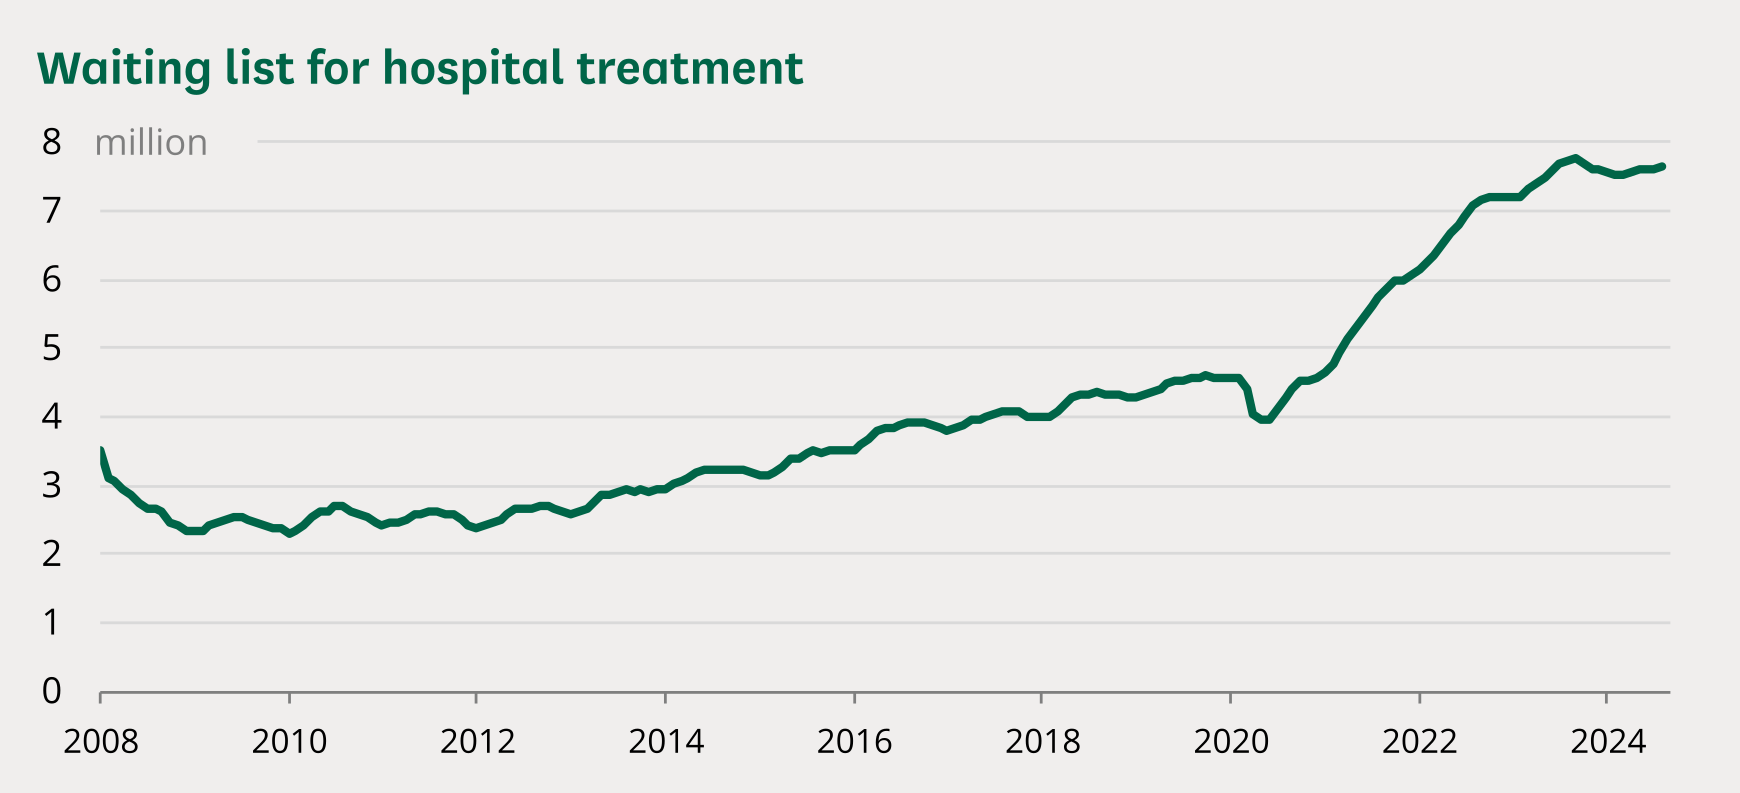
\includegraphics[width=1\linewidth]{img/Figuur-0.png}
    \caption{Wachtlijst van miljoenen patiënten voor ziekenhuisbehandeling (2011 - 2024)}
    \label{fig:Figuur0}
    \textit{Source: \autocite{Stiebahl2024}}
\end{figure}


%---------- Stand van zaken ---------------------------------------------------

\section{Literatuurstudie}%
\label{sec:literatuurstudie}

%Hier beschrijf je de \emph{state-of-the-art} rondom je gekozen onderzoeksdomein, d.w.z.\ een inleidende, doorlopende tekst over het onderzoeksdomein van je bachelorproef. Je steunt daarbij heel sterk op de professionele \emph{vakliteratuur}, en niet zozeer op populariserende teksten voor een breed publiek. Wat is de huidige stand van zaken in dit domein, en wat zijn nog eventuele open vragen (die misschien de aanleiding waren tot je onderzoeksvraag!)?

%Je mag de titel van deze sectie ook aanpassen (literatuurstudie, stand van zaken, enz.). Zijn er al gelijkaardige onderzoeken gevoerd? Wat concluderen ze? Wat is het verschil met jouw onderzoek?

% Verwijs bij elke introductie van een term of bewering over het domein naar de vakliteratuur, bijvoorbeeld~\autocite{Hykes2013}! Denk zeker goed na welke werken je refereert en waarom.

%Draag zorg voor correcte literatuurverwijzingen! Een bronvermelding hoort thuis \emph{binnen} de zin waar je je op die bron baseert, dus niet er buiten! Maak meteen een verwijzing als je gebruik maakt van een bron. Doe dit dus \emph{niet} aan het einde van een lange paragraaf. Baseer nooit teveel aansluitende tekst op eenzelfde bron.

%Als je informatie over bronnen verzamelt in JabRef, zorg er dan voor dat alle nodige info aanwezig is om de bron terug te vinden (zoals uitvoerig besproken in de lessen Research Methods).

% Voor literatuurverwijzingen zijn er twee belangrijke commando's:
% \autocite{KEY} => (Auteur, jaartal) Gebruik dit als de naam van de auteur
%   geen onderdeel is van de zin.
% \textcite{KEY} => Auteur (jaartal)  Gebruik dit als de auteursnaam wel een
%   functie heeft in de zin (bv. ``Uit onderzoek door Doll & Hill (1954) bleek
%   ...'')

%Je mag deze sectie nog verder onderverdelen in subsecties als dit de structuur van de tekst kan verduidelijken.


In de laatste decennia zijn de wachttijden voor de Accident and Emergency (A\&E) afdelingen binnen de National Health Service (NHS) substantieel toegenomen gekend zoals aangetoond in fig. \ref{fig:Figuur1}. Een recente onderzoeksbriefing uitgevoerd door \autocite{Baker2024} toont een sterke toename in de verhouding van patiënten die meer dan vier uur spenderen in de Accident and Emergency (A\&E) afdeling, en dit tussen 2015 en 2020. Sindsdien is er een nieuw record bereikt met 50,4\% van patiënten die meer dan vier uur doorbrengen in de Accident and Emergency (A\&E) afdeling. Dit vormt een duidelijke ondermijning van de vieruursnorm geïmplementeerd door de National Health Service (NHS). Deze richtlijn houdt in dat tenminste 95\% van de patiënten binnen vier uur moeten worden opgenomen, overgebracht en ontslagen worden. \autocite{NationalStatisticsONS2024}.

\begin{figure}[h]
    \centering
    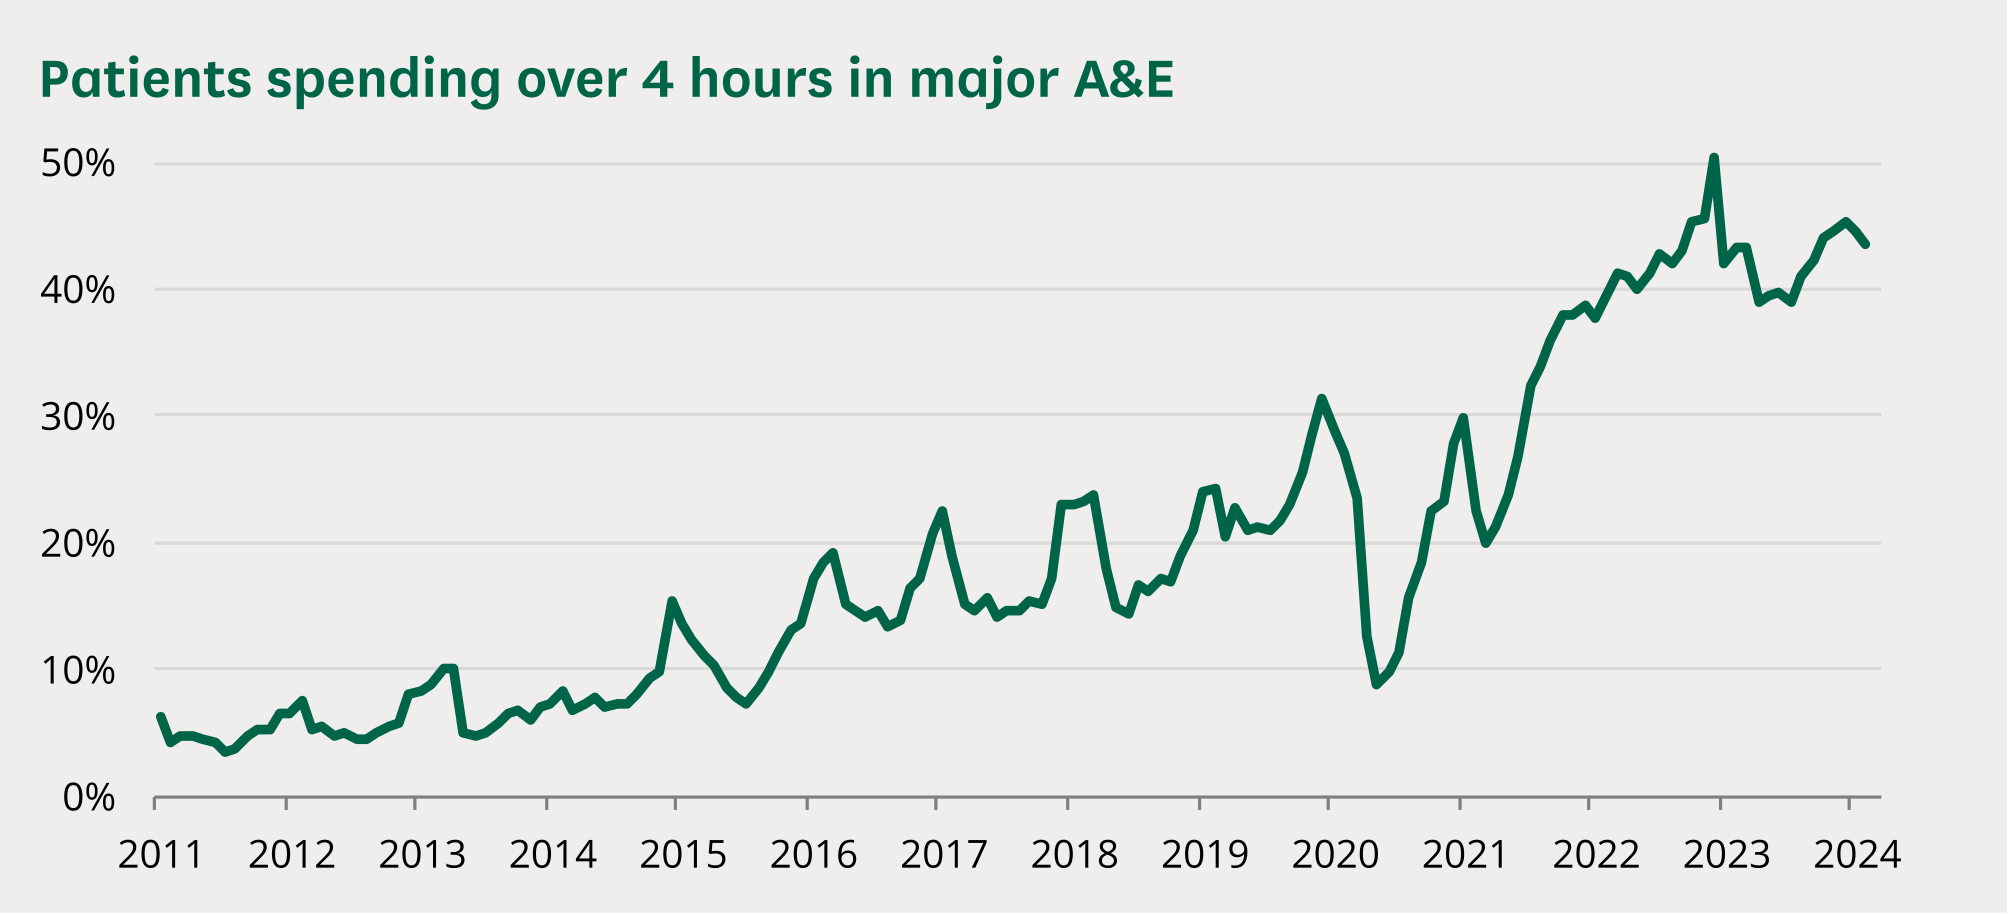
\includegraphics[width=1\linewidth]{img/Figuur-1.png}
    \caption{Percentage van patiënten die meer dan 4 uur spenderen in de Accident and Emergency (A\&E) departement}
    \label{fig:Figuur1}
    \textit{Source: \autocite{Baker2024}}
\end{figure}

Het niet voldoen aan deze richtlijn heeft serieuze gevolgen voor de zorgkwaliteit en patiëntentevredenheid zoals aangetoond door \autocite{Vainieri2020}. Volgens de bevindingen van \autocite{Paling2020} zijn de implicaties veel ernstiger. De studie vermeldt dat lange wachttijden in de Accident and Emergency (A\&E)-afdeling een verband toont met complicaties en mortaliteit onder patiënten. De oorzaak, volgens \autocite{Paling2020}, is te wijten aan een hoge beddenbezettingsgraad. Verder toont het onderzoek een correlatie tussen de hoge beddenbezetting  en de lange wachttijden in de Accident and Emergency (A\&E)-afdeling zoals aangetoond door fig. \ref{fig:Figuur2}.

\begin{figure}[h]
    \centering
    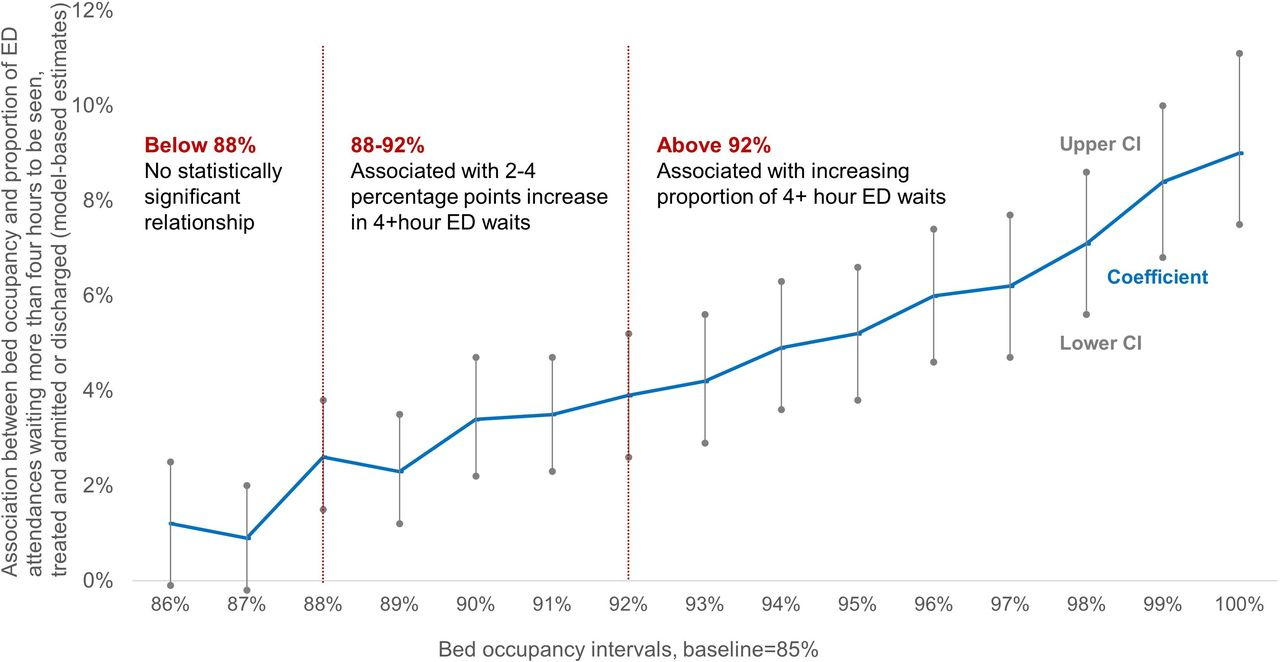
\includegraphics[width=0.5\textwidth]{img/Figuur-2}
    \caption{Plot dat een niet-lineaire relatie toont tussen bedbezettingen intervallen en proportie van patienten die meer dan 4 uur spenderen in de Accident and Emergency (A\&E) departement}
    \label{fig:Figuur2}
    \textit{Source: \autocite{Paling2020}}
\end{figure}

Patiënten zijn niet de enigen die worden beïnvloed door de langdurige wachttijden, onderzoekers hebben onlangs de werkomstandigheden van National Health Service (NHS)-werknemers onderzocht. De studie toont dat 40\% van alle ziektes bij het personeel te wijten is aan stress. Verder wijst het onderzoek uit dat de “overheersende stressfactor” veroorzaakt wordt door de hoge werkdruk \autocite{Ravalier2020}. \autocite{Vainieri2020} onderlijnt overbevolking als oorzaak van de hoge werkbelasting, en dit in Accident and Emergency (A\&E) departementen in diverse westerse landen. Om beter te begrijpen hoe Internet of Things (IoT) dit probleem kan oplossen, is het noodzakelijk om dieper in te gaan op wat Internet of Things (IoT) precies inhoudt. Over het algemeen verwijst Internet of things (IoT) naar een model dat verschillende technologieën omvat. Anders gezegd, is het een netwerk van elektronische apparaten die met elkaar of met de cloud communiceren via het internet. De afgelopen twee decennia hebben een grote invloed gehad op de snelle vooruitgang van Internet of Things (IoT) \autocite{Almutairi2024}, hierdoor is het aantal aangesloten Internet of Things (IoT)-devices sterk gestegen, met 7.74 miljard in 2019, 10.7 miljard in 2021 \autocite{Dawod2022} en 25.44 miljard tegen 2030 \autocite{Dawod2022}. Sensoren, camera's en gelijkaardige apparaten worden al “geïntegreerd” in “woningen” en “voertuigen” \autocite{Dawod2022} en geïmplementeerd over verschillende sectoren zoals de “gezondheidszorg, landbouw, productie” en slimme steden \autocite{Almutairi2024}.

De implementatie van miljarden \autocite{Dawod2022} Internet of Things (IoT)-devices over verschillende sectoren geeft een duidelijk representatie van de veranderingen die Internet of Things (IoT) zal brengen over de manier waarop men leeft, werkt en omgaat met de omgeving \autocite{Almutairi2024}. De vraag is nu of Internet of Things (IoT) gebruikt kan worden in de gezondheidszorg om wachttijden in de Accident \& Emergency departementen te verkorten. Volgens een recente studie uitgevoerd door \autocite{Singh2023} is het perfect mogelijk om Internet of Things (IoT) te implementeren in de gezondheidszorg. Echter, concludeert het onderzoek dat Internet of Things (IoT) een gunstige invloed heeft en dit ondanks de beperkingen in “energie, processing en opslag”. Verder benadrukt de studie dat Internet of Things (IoT) een “veelbelovende technologie” is bij het sparen van tijd en moeite voor het medische personeel. 

%----------------------------------------------------------------------------------------------------------------------

Internet of Things (IoT) kan op verschillende manieren worden ingezet in de gezondheidszorg \autocite{Huang2021}. Ten eerste kan Internet of Things (IoT) toegepast worden voor het beheren van medische uitrusting, medicatie en data. Vervolgens door gebruik te maken van Internet of Things (IoT)-ondersteunende slimme apparaten en systemen kan de patiënten stroom worden beheerd \autocite{Almotaira2023} en patiënten pieken voorspeld \autocite{King2022}. De werking hiervan, zoals aangetoond in fig. \ref{fig:Figuur4} is als volgt, iedere patiënt beschikt over zijn eigen Internet of Things (IoT)-device, zoals een sensor of een netwerk device. De device is vervolgens verbonden met een intelligente gateway, ook wel Internet of Things (IoT)-gateway genoemd. Deze gateway zorgt voor communicatie tussen devices, en tussen device en cloud \autocite{Upadrista2021}. De gateway is verbonden met een datacollectie- en processing center via het internet, deze is verantwoordelijk voor het verwerken van ruwe data door het “correctheid” en “kwaliteit” te verbeteren om deze geschikt voor analyse te maken \autocite{Sirisha2023}. Eenmaal de ruwe data verwerkt, worden deze geanalyseerd en maakt het systeem beslissingen, die vervolgens door artsen en dokters gebruikt kunnen worden \autocite{Singh2023}. Kortom, verzamelen Internet of Things (IoT)-apparaten realtime patiëntgegevens die geanalyseerd zijn om inzichten te maken en trends te voorspellen \autocite{Alrehaili2023, Sidhu2023}. 

\begin{figure}[h]
    \centering
    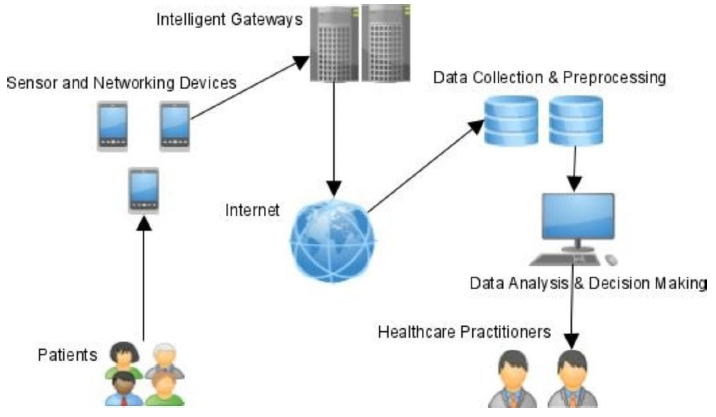
\includegraphics[width=0.5\textwidth]{img/Figuur-4}
    \caption{Internet of things (IoT) systeem in de gezondheidszorg}
    \label{fig:Figuur4}
    \textit{Source: \autocite{Singh2023}}
\end{figure}


%---------- Methodologie ------------------------------------------------------
\section{Methodologie}%
\label{sec:methodologie}

% Hier beschrijf je hoe je van plan bent het onderzoek te voeren. Welke onderzoekstechniek ga je toepassen om elk van je onderzoeksvragen te beantwoorden? Gebruik je hiervoor literatuurstudie, interviews met belanghebbenden (bv.~voor requirements-analyse), experimenten, simulaties, vergelijkende studie, risico-analyse, PoC, \ldots?

% Valt je onderwerp onder één van de typische soorten bachelorproeven die besproken zijn in de lessen Research Methods (bv.\ vergelijkende studie of risico-analyse)? Zorg er dan ook voor dat we duidelijk de verschillende stappen terug vinden die we verwachten in dit soort onderzoek!

% Vermijd onderzoekstechnieken die geen objectieve, meetbare resultaten kunnen opleveren. Enquêtes, bijvoorbeeld, zijn voor een bachelorproef informatica meestal \textbf{niet geschikt}. De antwoorden zijn eerder meningen dan feiten en in de praktijk blijkt het ook bijzonder moeilijk om voldoende respondenten te vinden. Studenten die een enquête willen voeren, hebben meestal ook geen goede definitie van de populatie, waardoor ook niet kan aangetoond worden dat eventuele resultaten representatief zijn.

%Uit dit onderdeel moet duidelijk naar voor komen dat je bachelorproef ook technisch voldoen\-de diepgang zal bevatten. Het zou niet kloppen als een bachelorproef informatica ook door bv.\ een student marketing zou kunnen uitgevoerd worden.

% Je beschrijft ook al welke tools (hardware, software, diensten, \ldots) je denkt hiervoor te gebruiken of te ontwikkelen.

%Probeer ook een tijdschatting te maken. Hoe lang zal je met elke fase van je onderzoek bezig zijn en wat zijn de concrete \emph{deliverables} in elke fase?

Dit onderzoek heeft als doel het verminderen van wachttijden op de Accident and Emergency (A\&E) afdelingen van de National Health Service (NHS) in Engeland door middel van Internet of Things (IoT).


\subsubsection*{Oorzaakanalyse}
Het onderzoek begint met het uitvoeren van een uitgebreide oorzaakanalyse, dit is een fundamentele stap bij het identificeren van de oorzaak van de langdurige wachttijden binnen de A\&E-afdelingen van de National Health Service (NHS). De analyse begint met het definiëren van het probleem, om die reden zal de 5 Whys”-methode toegepast worden samen met een brainstorming-sessie. De 5 Whys”-method is gebruikt om de kern van het probleem te achterhalen en dit door elke keer de vraag waarom te stellen, \ref{fig:Figuur5} en de oorzaak proberen te identificeren via de brainstorming-sessie. Zodra diverse oorzaken geïdentificeerd zijn, begint er een analyse door middel van het Fishbone-model. De reden achter het gebruik van dit model is het voorkomen dat mogelijke onderliggende oorzaken over het hoofd worden gezien. Verder biedt het model simpliciteit bij het trekken van conclusies dankzij een visuele representatie tussen de categorisch weergegeven oorzaken en het probleem. Vervolgens is elke oorzaak zorgvuldig bestudeerd, degene die de grootste impact heeft op langdurige wachttijden is geselecteerd als de hoofdoorzaak. Een overweging is vervolgens gemaakt, om te achterhalen of IoT in het algemeen een oplossing kan zijn voor deze oorzaak. Verder in het onderzoek wordt er dieper bekeken naar welke IoT-devices gebruikt kunnen worden in de gezondheidszorg, zodra de devices geselecteerd zijn, wordt er op een meer diepgaande wijze bekeken hoe de apparaten een oplossing kunnen zijn voor de hoofdoorzaak.

\begin{figure}[h]
    \centering
    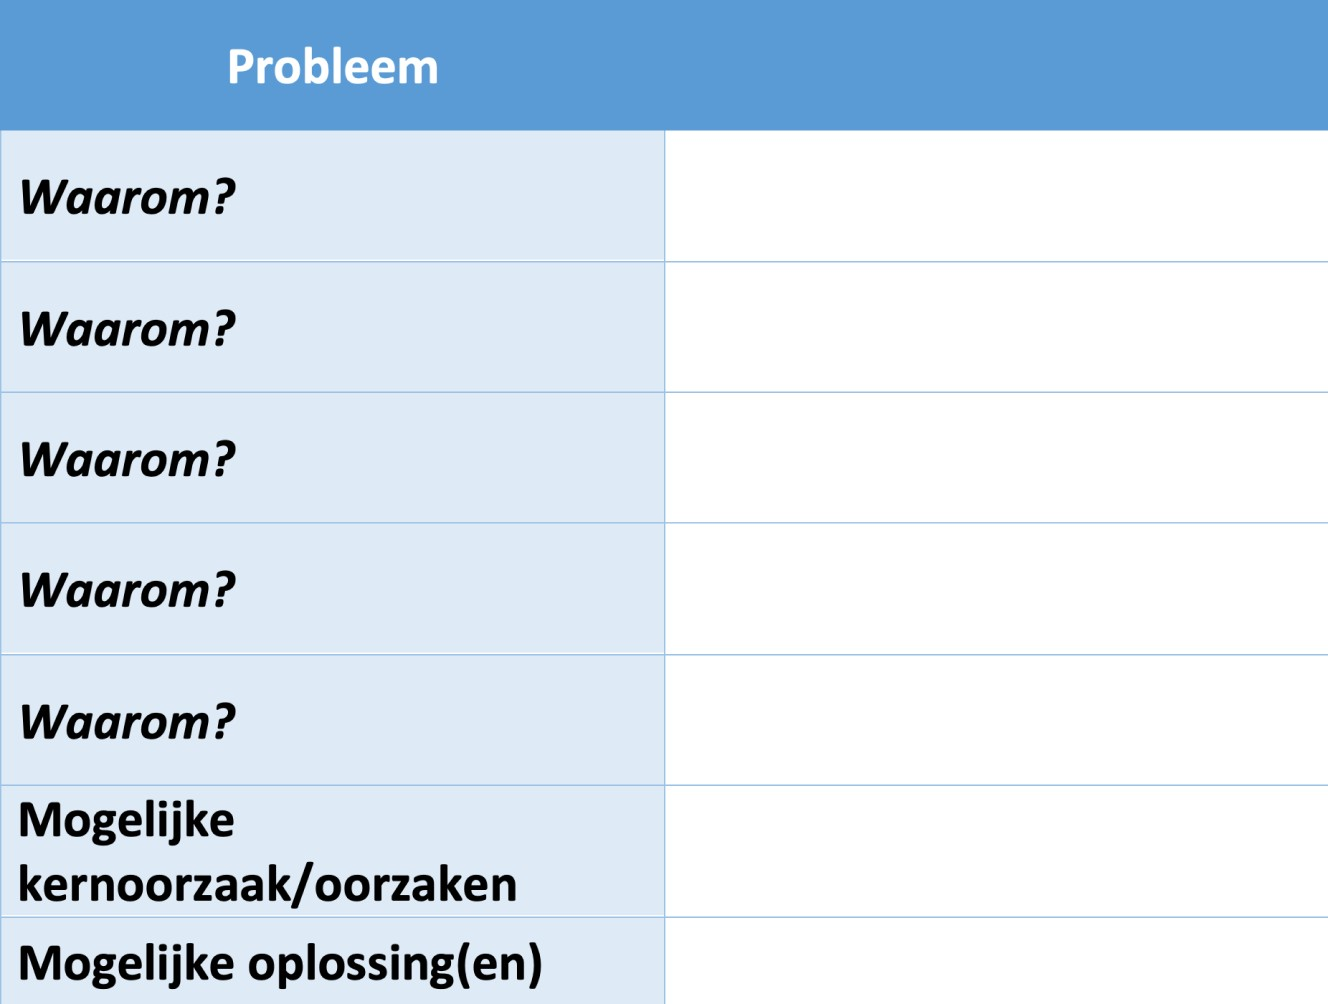
\includegraphics[width=0.5\textwidth]{img/Figuur-5}
    \caption{5 Whys”-method}
    \label{fig:Figuur5}
    \textit{Source: \autocite{Scharwaechter2023}}
\end{figure}

\begin{figure}[h]
    \centering
    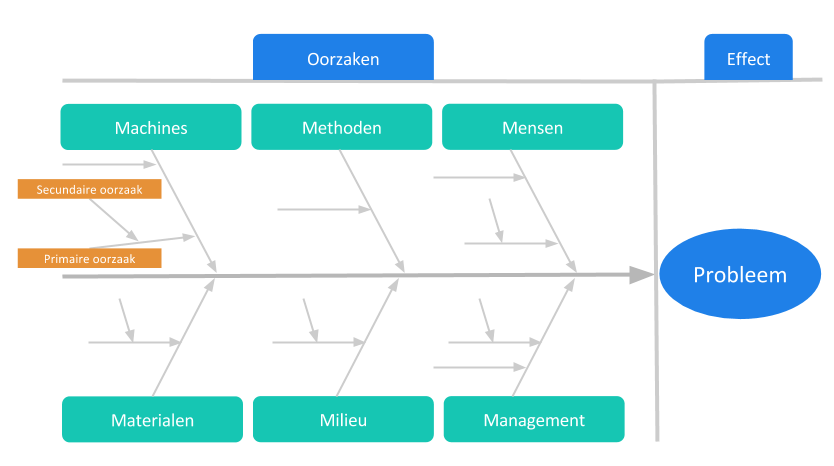
\includegraphics[width=0.5\textwidth]{img/Figuur-6}
    \caption{The fishbone diagram (also called the Ishikawa diagram)}
    \label{fig:Figuur6}
    \textit{Source: \autocite{Swaen2023}}
\end{figure}


%Een oorzaakanalyse is een belangrijk onderdeel van deze onderzoek, voor die reden wordt er een uitgebreide analyse uitgevoerd voor het identificeren oorzaak van de langdurige wachttijden binnen de A\&E-afdelingen van de National Health Service (NHS)

\subsubsection*{Gegevensverzameling}
Het verzamelen van informatie begint met het identificeren van diverse Na-tio-nal Health Ser-vice zie-ken-hui-zen
met de meest uitgebreide wachttijden in de Accident and Emergency (A\&E). Het doel van deze gegevensverzameling is het vaststellen van Na-tio-nal Health Ser-vice zie-ken-hui-zen met uitgebreide Accident and Emergency (A\&E) wachttijden, aangezien deze gegevens essentieel zijn voor de selectieprocedure en simulaties die in de volgende secties aan bod komen. Relevante gegevens worden geselecteerd door verschillende bronnen te raadplegen zoals NHS Digital, NHS UK. De bronnen worden gekozen op basis van hun relevantie voor het onderzoek en datum van publicatie daarvan. Deze datum moet zo recent mogelijk zijn om een representatief beeld te kunnen geven van de huidige toestand, daarvoor zullen enkel gegevens van de laatste maand (maart 2024) behouden worden. De informatie is geselecteerd met als voorwaarde dat deze in CSV-formaat beschikbaar is. Dit formaat maakt het bestand makkelijk aanpasbaar door gebruik te maken van Python wat praktisch is tijdens het verwerken van het bestand. De gegevens dienen ook de naam van de ziekenhuizen te bevatten alsook kwantitatieve gegevens over wachttijden in de Accident and Emergency (A\&E). Dit onderzoek richt zich enkel op ziekenhuizen in Engeland waardoor de namen zeer belangrijk zijn. Als laatste dienen de gegevens een onderscheid te tonen tussen de wachttijden minder dan vier uur en deze meer dan vier wat noodzakelijk is bij het vaststellen van langdurige wachttijden. Na het verzamelen van de nodige gegevens over de National Health Service (NHS)-ziekenhuizen, is het literatuurstudie \ref{sec:literatuurstudie} geraadpleegd voor informatie over de gebruikte Internet of Things (IoT)-devices in Accident and Emergency (A\&E) afdelingen. De verzamelde informatie zal vervolgens gebruikt zijn in de toekomstige simulatie over de gekozen ziekenhuis in de selectieprocedure.

\subsubsection*{Gegevensverwerking en Selectieprocedure}
Python, Numpy en Pandas zijn tools die worden gebruikt voor het verwerken van het dataframe, deze tools zijn gebruikt voor het uitfilteren van de onnodige gegevens. Als eerste wordt de gegevensstructuur geanalyseerd zijn voor het identificeren van de te selecteren kolommen en rijen. Enkel kolommen die gegevens bevatten over het datum en ziekenhuis zijn behouden.

Het dataframe wordt vervolgens gebruikt in de selectieprocedure. Deze procedure houdt in dat een ziekenhuis aan diverse voorwaarden moet voldoen om geselecteerd te zijn, deze criteriums houden in dat een ziekenhuis gelegen moet zijn in Engeland. Verder zijn de ziekenhuizen die nul of geen waarde hebben voor wachttijden over de vier uur niet behouden. het ziekenhuis met de meeste patiënten in de kolom met wachttijden over de 4 uur is geselecteerd.

\subsubsection*{Case study}
Deze case study wordt gerealiseerd als toelichting voor het implementeren van Internet of Things (IoT)-technologieën en dit met als doel om wachttijden in de Accident and Emergency (A\&E) afdelingen van de National Health Service (NHS) te verkorten. De primaire doelstelling van deze case study is het identificeren van praktische voorbeelden van Internet of Things (IoT)-gebruik om lange wachttijden in Accident and Emergency (A\&E)-afdelingen te verminderen. Daarnaast richt de case study zich op het identificeren van verschillende Internet of Things (IoT)-apparaten die ingezet kunnen worden om wachttijden verder te verkorten. De case study begint met het identificeren specifieke casussen. In het geval van deze onderzoeksvraag dienen deze te voldoen aan diverse criteria, deze houden in dat een casus over een bepaald ziekenhuis dient te voldoen aan de criteria, welke zijn vastgesteld in het selectieprocedure, met uitzondering van de locatie. Bovendien dient de gekozen casus, in dit geval één of meerdere ziekenhuizen gebruik maken van Internet of Things (IoT) in Accident and Emergency (A\&E) afdelingen bij het bestrijden van langdurige wachttijden. Na het vast stellen van een casus worden er kwalitatieve en kwantitatieve gegevens verzameld over de gekozen casus, dit houdt in dat verschillende bronnen worden geraadpleegd bij het verzamelen van informatie zoals, wetenschappelijke literatuur, rapporten van gezondheidsorganisaties, archieven en documenten. Een voorbeeld van deze bronnen zijn National Library of Medicine. Na het vaststellen van diverse casussen worden deze vergeleken met het ziekenhuis uit de selectieprocedure, de casus die het meest overeenstemt met de geselecteerde ziekenhuis wordt gekozen. De casus wordt vervolgens geanalyseerd en de gebruikte Internet of Things (IoT)-devices en Internet of Things (IoT)-categorieën opgelijst, verder worden gegevens verzamelt voor elk van de opgelijste devices, verschillende bronnen zoals onderzoeksrapporten, literatuurstudies, academische tijdschriften en technologische onderzoeken worden hiervoor geraadpleegd. De verzamelde gegevens worden vervolgens geanalyseerd met als doel een beter begrip te krijgen over hoe deze in de casus geïmplementeerd zijn en hoe deze toegepast kunnen worden in de geselecteerde ziekenhuis. 


\subsubsection*{Identificeren van IoT-devices}
Het identificeren van IoT-apparaten is van het uiterste belang, daarom is er aanzienlijk veel tijd besteed bij het opstellen van de casestudie om een assortiment van IoT-apparaten te bepalen. Dit houdt in dat elk apparaat grondig bestudeerd zal zijn om een beter begrip te krijgen in de werking hiervan in de gezondheidszorg. Om het meest gepaste IoT-apparaat te selecteren worden verschillende IoT-categorieën bekeken, deze categorieën vertegenwoordigen IoT-apparaten die de werking van de A\&E-departementen kan verbeteren en efficiënter maken, deze categorieën zijn: Locatie- en traceerapparaten, Communicatieapparaten, Geautomatiseerde medicatie dispensers, Integratie van het gegevensbeheer en Integratie en coördinatie van IoT-devices.

De eerste geselecteerde device(s) zijn de RFID-Tags vanuit de Location and Tracking categorie, deze tags zullen ingezet zijn voor het opsporen van patiënten, uitrusting en personeel op de werkvloer, dit IoT-device zorgt ervoor dat alles makkelijk te vinden is, waardoor het personeel zich volledig kan focussen op binnenkomende patiënten.

Verder zullen er Smart Tablets and Displays en Patient Kiosks ingezet zijn, deze behoren tot de categorie Communication Devices, de Smart Tablets and Displays zorgen ervoor dat het personeel in staat zijn om realtime gegevens, waarschuwingen en patiëntinformatie kan ontvangen van patiënten op de spoeddienst. Het gebruik van Smart Tablets and Displays zorgt ervoor dat het personeel steeds beschikt over de meest recente gegevens wat van uiterst belang is bij het verzorgen van patiënten. Daarnaast zullen er Patient Kiosks ingeschakeld zijn, patiënten kunnen deze gebruiken om check-ins of updates te krijgen over de wachttijden en de volgende onderzoeken.

Vervolgens zullen slimme medicijnkastjes en pillendispensers ingeschakeld zijn, de slimme medicijnkastjes zullen gebruikt zijn om het uitgave van medicatie efficiënter te maken dankzij verschillende geautomatiseerde aspecten. Daarnaast zal er een device gebruikt zijn als gecentraliseerde data systeem, of een Central Data Hub, dit IoT-apparaat vereist dat gegevens opgeslagen worden op een centrale locatie, dit zorgt ervoor dat dezelfde patiëntengegevens toegankelijk zijn door het volledige personeel zonder dat de gegevens uit verschillende systemen moeten worden gehaald. Als laatste zal er een IoT Platform samen met een AI and Analytics software ingezet zijn, deze platform is een centrale platform om alle IoT-devices te verbinden, monitoren and beheren, deze zorgt ervoor dat alle devices correct samen werken. De software daarentegen zal gebruikt worden om de data vanuit de IoT-devices te analyseren om vervolgens voorspellingen te maken over de patiëntenstroom en triage benodigdheden.

\subsubsection*{Het gebruik van Machine Learning, Predictive Analytics en synthetische IoT data}
Het complementaire gebruik van Ma\-chi\-ne Lear\-ning, Predictive Analytics en synthetische IoT-\-ge\-ge\-vens is de gekozen methode om te illustreren of Internet of Things (IoT) een gunstig effect heeft op het terugdringen van lange wachttijden voor de National Health Service (NHS). Deze keuze is gemaakt vanwege de vele uitdagingen om dit in de werkelijkheid te testen. Kortom, zijn er nog veel drempels bij het uitvoeren van gelijkaardige testen, vooral in National Health Service (NHS)-ziekenhuizen. Daardoor wordt er gekozen om gebruik te maken van Machine Learning, Predictive Analytics en synthetische IoT-gegevens om aan te tonen dat IoT een gunstige invloed heeft bij het verkorten van langdurige wachttijden. Om dit doel te vervullen zijn de Machine Learning en Predictive Analytics algoritmes eerst en vooral getraind, en dit door middel van verzamelde historische gegevens en synthetische IoT data. Verder volgt er de generatie van de synthetische IoT data voor elk IoT device door middel van Python en Python libraries zoals Pandas, Numpy en Faker. De synthetische data bevat gegevens over de diverse verplaatsingen van patiënten binnen de A\&E en de tijd die op elke locatie doorgebracht zijn. Eenmaal de algoritmes getraind kan het model gebruikt worden om wachttijden te voorspellen tijdens de patiëntenflow \ref{fig:Figuur6} voor diverse scenario's zoals veranderingen in het aantal patiënten en personeel. Tot slot worden de wachttijden voor de diverse scenario's vergeleken met de historische data en worden er conclusies getrokken en de onderzoeksvraag beantwoord.

\begin{figure}[h]
    \centering
    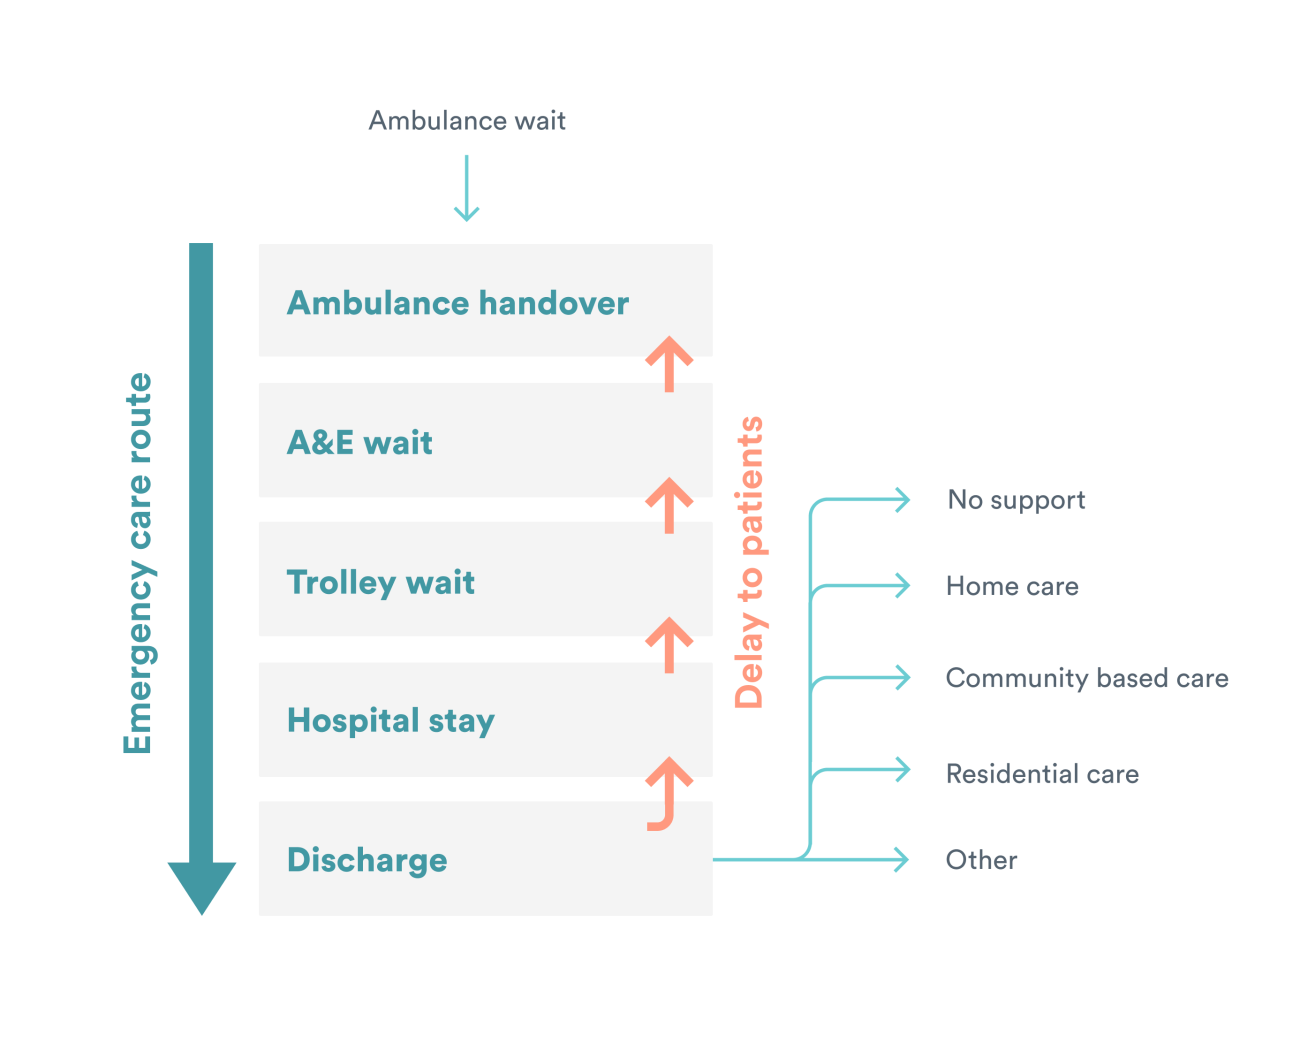
\includegraphics[width=0.5\textwidth]{img/Figuur-7}
    \caption{Patiëntenflow A\&E}
    \label{fig:Figuur7}
    \textit{Source: \autocite{Morris}}
\end{figure}

\subsubsection*{Resultaten}

De resultaten worden beschouwd als een succes, indien de voorspellingen duidelijk aan tonen dat er een significant vermindering is in de wachttijden na het gebruik van Internet of Things (IoT). Dit gebeurt door de voorspellingen te vergelijken met de historische data, hieruit worden conclusies getrokken

De bevindingen met betrekking tot de voorspellingen worden vergeleken met de historische data, de waarnemingen die daaruit volgen worden vervolgens geanalyseerd in de context van potentiële voordelen van Internet of Things (IoT) met betrekking tot de uitgebreide Accident and Emergency (A\&E) wachttijden. De resultaten van het onderzoek lichten verder toe of Internet of Things (IoT) kan bijdragen bij het verminderen van wachttijden voor de Accident and Emergency (A\&E) afdeling door gebruik te maken van technologieën uit verschillende IoT categorieën. Als er voldoende aanwijzingen zijn dat Internet of Things (IoT)-tech\-no\-lo\-gieën een gunstige invloed hebben op de wachttijden binnen de Accident and Emergency (A\&E) afdeling, dan zijn de resultaten als succesvol gewaardeerd.


\subsubsection*{Milestone}

\begin{figure}[h]
    \centering
    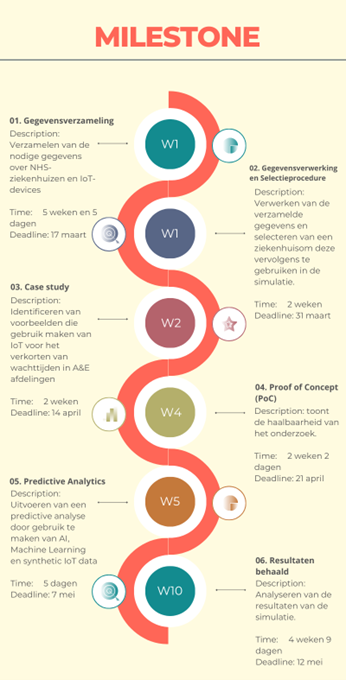
\includegraphics[width=0.93\linewidth]{img/milestone-2.png}
    \label{fig:Figuur8}
\end{figure} 

%---------- Verwachte resultaten ----------------------------------------------
\section{Verwacht resultaat, conclusie}%
\label{sec:verwachte_resultaten}

Hier beschrijf je welke resultaten je verwacht. Als je metingen en simulaties uitvoert, kan je hier al mock-ups maken van de grafieken samen met de verwachte conclusies. Benoem zeker al je assen en de onderdelen van de grafiek die je gaat gebruiken. Dit zorgt ervoor dat je concreet weet welk soort data je moet verzamelen en hoe je die moet meten.

Wat heeft de doelgroep van je onderzoek aan het resultaat? Op welke manier zorgt jouw bachelorproef voor een meerwaarde?

Hier beschrijf je wat je verwacht uit je onderzoek, met de motivatie waarom. Het is \textbf{niet} erg indien uit je onderzoek andere resultaten en conclusies vloeien dan dat je hier beschrijft: het is dan juist interessant om te onderzoeken waarom jouw hypothesen niet overeenkomen met de resultaten.



\printbibliography[heading=bibintoc]

\end{document}